\section{Amplificatore di potenza e preamplificatore}
	Si è proceduto al montaggio del circuito in \figurename{ \ref{fig:ampli}}
	impiegando le corrispondenti componentistiche.
	\begin{figure}[htb]
		\begin{minipage}{0.75\textwidth}
		\centering
		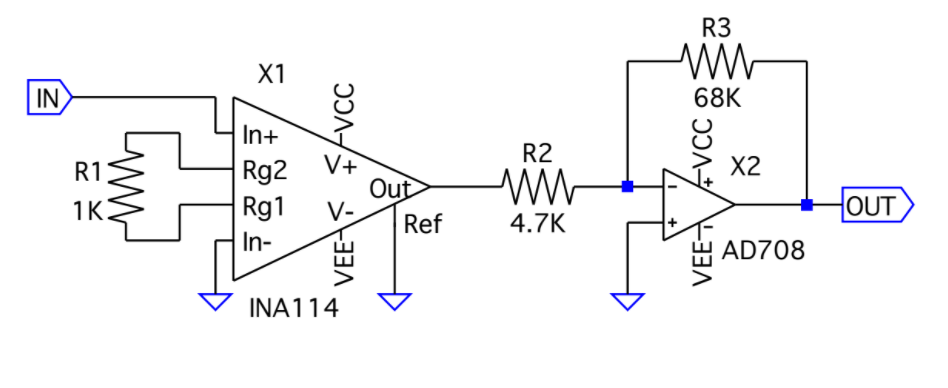
\includegraphics[scale=0.4]{ampli.png}
		\caption{Circuiti amplificatore di potenza e preamplificatore.}
		\label{fig:ampli}
		\end{minipage}
			\begin{minipage}{0.19\textwidth}
			\begin{tabular}{l@{ }c@{ }l}
				$R_{1}$& = &\SI{9.78\pm 0.08}{\kilo\ohm}\\
				$R_{2}$& = &\SI{1.5\pm0.1}{\kilo\ohm}\\
				$R_{3}$& = &\SI{80.8\pm0.7}{\kilo\ohm}\\
				$R_{4}$& = &\SI{56.6\pm0.6}{\kilo\ohm}\\
				$R_{5}$& = &\SI{18.1\pm0.2}{\kilo\ohm}\\
				$R_{6}$& = &\SI{119(1)}{\kilo\ohm}\\
				$R_{7}$& = &\SI{3.83\pm0.04}{\kilo\ohm}\\
				$R_{9}$& = &\SI{1.30\pm0.01}{\mega\ohm}\\
			
				
				
				$C_1$& = &\SI{114(5)}{\nano\farad}\\
				$C_2$& = &\SI{114.8(5)}{\nano\farad}
		\end{tabular}
		\end{minipage}
	\end{figure}
	Si è proceduto successivamente alla verifica del comportamento circuitale.
	Per fare ciò si è proceduto ad acquisire la forma d'onda misurabile in $S6$
	ottenendo le acquisizioni in \figurename{ \ref{fig:S6}};
	\begin{figure}[h]
		\centering
		\subfloat[S6 non schermato]{
			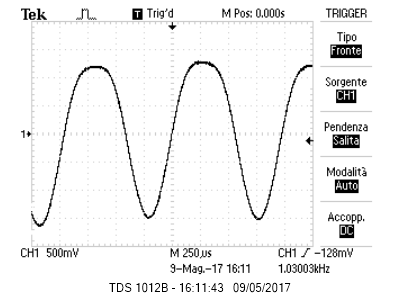
\includegraphics[scale=0.5]{led-rumoroso.png}
			\label{fig:S6a}
		}
		\qquad
		\subfloat[S6 schermato da luce ambientale ch. 2]{
			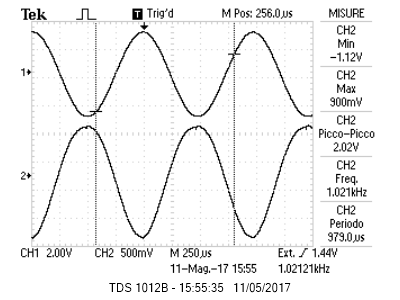
\includegraphics[scale=0.5]{s6-vuoto.png}
			\label{fig:S6b}
		}\\
		\subfloat[S6 con 2 lastre ch.2]{
			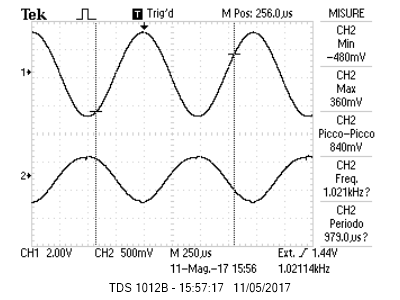
\includegraphics[scale=0.5]{s6-2-piastre.png}
			\label{fig:S6c}
		}
		\qquad
		\subfloat[rumore luce ambientale]{
			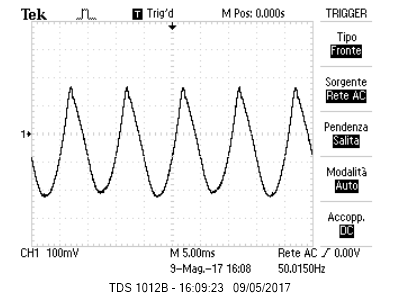
\includegraphics[scale=0.5]{rumore-50-hz.png}
			\label{fig:S6d}
		}\\
		\caption{Acquisizione delle forme d'onda osservate su S6}
		\label{fig:S6}
	\end{figure}
	come è possibile vedere da tali acquisizioni il segnale S6 in presenza di luce diffusa
	nell'ambiente di lavoro presenta una forma d'onda solo approssimativamente sinusoidale (\figurename{ \ref{fig:S6a}}); schermando tale segnale
	si ottiene $V_{pp}= $\SI{2.02\pm 0.04}{\volt} ed una forma d'onda che corrisponde maggiormente ad una
	sinusoidale \figurename{ \ref{fig:S6b}}.
	Si è pertanto proceduto a inattivare il diodo LED e acquisire il segnale provocato
	dalla luminosità
	diffusa nel ambiente di lavoro ottenendo un segnale
	di $V_{pp_{noise}}$ dell'ordine di \SI{400}{\milli \volt}\footnote{La $f$ rilevata $f\sim $\SI{50}{\hertz} è la frequenza
	della tensione di rete.}; tale segnale di $noise$ risulta compatibile con i segnali
	ottenuti frapponendo già $2$ lastre di mylar,$V_{pp}= $\SI{840 \pm 8}{\milli \volt} (\figurename{ \ref{fig:S6c}}).
	A seguito di questa verifica preliminare si è stato ritenuto necessario montare il
	circuito completo in \figurename{ \ref{f:complessivo} per scermare il sistema da
	i rumori ambientali.
